\documentclass[11pt]{article}
\usepackage[margin=2.2cm]{geometry}
\usepackage[T1]{fontenc}
\usepackage{amsmath,amssymb,booktabs,graphicx,xcolor,enumitem,caption,longtable,array}
\usepackage[section]{placeins}
\usepackage{hyperref}
\usepackage{xurl}
\usepackage{fvextra}
\fvset{breaklines=true,fontsize=\footnotesize}
\setlist{itemsep=2pt,topsep=3pt}
\hypersetup{colorlinks=true,linkcolor=blue!50!black,urlcolor=blue!50!black}
\captionsetup{font=small,labelfont=bf}
\setlength{\emergencystretch}{3em}

\title{The v3 data set: the voltages, and how much each parameter moves the noise and the dark current}
\author{ccd\_opt\_ml, level 1}
\date{Plan of 2026-11-10, after the v2 analysis}

\begin{document}
\maketitle

\section*{Summary}
The v2 data (sessions D, E) showed that the dark charge $\lambda$ is set mainly by the \emph{timing}: $\lambda$ rises with
the readout time ($\lambda \propto \texttt{delayInt}^{\,0.5}$ on every amplifier; its dark-current part is linear in the
skip-cycle time), and a settings-only model already gets the direction of almost every $\lambda$ change right. That part
is simple physics. What v2 could not resolve is the more subtle question of how the \emph{voltages} move the dark current:
every clock voltage moved by at most 0.5\,V, in locked groups, and always together with a timing change.

v3 is a voltage-focused data set: 152 packets on board 101 (about 42\,h) in two sessions, G (123 packets, training) and
H (29 packets, the prospective test). 72 of the 123 training packets change \emph{only voltages} at nominal timing; the
voltages move independently (each clock phase on its own, the clock swings for the first time) over their voltage
windows, with every configuration, and every intermediate state of applying it and of returning to nominal, inside the
group's relationship rules with a margin of at least 0.5\,V, and every clock swing at least 1.5\,V.

The data serve two goals:
\begin{enumerate}
\item \textbf{(new) Quantify how much each parameter moves the noise ($\sigma_e$) and the dark current ($\lambda$)}, with
  uncertainties: per-volt effects, their share of the variance, interactions, how they differ between amplifiers, and
  for $\lambda$ whether a voltage changes the dark-current \emph{rate} or the \emph{clock-induced charge}.
\item \textbf{Keep training and testing the level-1 models}, now on changes at fixed timing, where they are weakest.
\end{enumerate}

\section{Where the project stands after v2}

\subsection{The models}
\begin{itemize}
\item \textbf{Absolute (Task A), session E, frozen models:} $\sigma_e$ 9.0\,\% typical error (mean 22.2\,\%, settings only
  17.1\,\%); on a new amplifier the trace physics model gets 9.7\,\% against 18.1\,\% from the settings (significant).
  $\lambda$ 28.6\,\% (settings + amplifier 21.1\,\%: the traces add nothing); on a new amplifier $\lambda$ is not
  predicted (50--90\,\%). Gain 1.7\,\% (same as the settings).
\item \textbf{Change models (Task B), new amplifiers:} the direction of clear $\sigma_e$ changes 88\,\% on session E
  (frozen direction classifier; settings only 72\,\%), size error 13\,\% against 28--29\,\%. The pass mark (raised to
  90\,\%) is missed by 2 points; session E is too small (about 15 packets) for most differences to be significant.
  $\lambda$ and gain directions 94--99\,\%, but the settings alone get the same.
\item \textbf{Where the models are weak:} when \texttt{delayInt} does not change, the $\sigma_e$ direction falls from
  86--92\,\% to about 74\,\% for every model (settings only 60\,\%). Session E had no such pairs. These are exactly the
  changes v3 is made of.
\item \textbf{Session E $\lambda$:} the large $\lambda$ errors on E come from one packet, L2\_72 (\texttt{delayRGH} and
  VSUB both at their maximum, long \texttt{delayInt}): $\lambda$ 80\,\% above the settings model on every amplifier.
  Without it the E $\lambda$ change errors are 13--15\,\%, as on D. An interaction in an unsampled corner.
\end{itemize}

\subsection{What v2 says about the parameters}
\begin{itemize}
\item \textbf{$\lambda$ is a timing quantity first} (Fig.~\ref{fig:importance}): a settings-only model explains 91\,\% of the
  variance of $\lambda$ changes; \texttt{delayInt} carries almost all of it, then \texttt{delayRGH} and VSUB. Each
  amplifier sits at its own level, but the lines are parallel (Fig.~\ref{fig:lambdaknobs}): an amplifier's offset cancels
  in a change, which is why the change models transfer to a new amplifier and the absolute $\lambda$ models do not.
\item \textbf{With the timing removed, $\lambda$ still varies by 9.3\,\% RMS} (label noise about 2.5\,\%), so there are
  real voltage effects. Almost all of it is VSUB (Fig.~\ref{fig:volts}): about $+8$ to $+12$\,\% per 2.5\,V on ch1 and
  ch3, nearly nothing on ch0 and ch2. Every other voltage is below 1.5\,\% per standard deviation, but those were moved
  over 0.5--1\,V only, in locked groups (V1/V2/V3 lows together, H1/H2/H3 lows together, the highs never): their effects
  cannot be resolved or told apart in v2.
\item \textbf{What transfers between amplifiers} (Fig.~\ref{fig:transfer}): the timing effects agree on all four
  amplifiers; VSUB is the one knob whose effect is as large between amplifiers as its shared part. A change model
  meets this on a new amplifier: an estimated 6\,\% error on $\lambda$ changes, 2\,\% on $\sigma_e$, 0.3\,\% on gain.
\item \textbf{$\sigma_e$} is driven by \texttt{delayInt} with a strong non-linearity (white noise falls with a longer
  window, slow noise grows: Sobol interaction share 0.53), then V1/V2 lows, \texttt{delayRGH}, VSUB and SW\_L at a few
  \% per standard deviation each. The traces see $\sigma_e$ directly (it is a readout noise), which is why the trace
  models win on $\sigma_e$ and not on $\lambda$.
\item \textbf{Dark rate and clock-induced charge.} Fitting
  $\lambda = t^{\alpha} e^{r} + e^{c}$ ($t$ the skip-cycle time) on v2 gives $\alpha = 1.02 \pm 0.18$ and 13--25\,\% of
  $\lambda$ from clock-induced charge at nominal. Which voltage changes which term is not constrained by v2 (the voltages
  were never varied at several fixed timings); v3 is built to measure it.
\item Gain is set by VR and VDD (the output stage); nothing else matters at the 0.1\,\% level.
\end{itemize}

\begin{figure}[ht]\centering
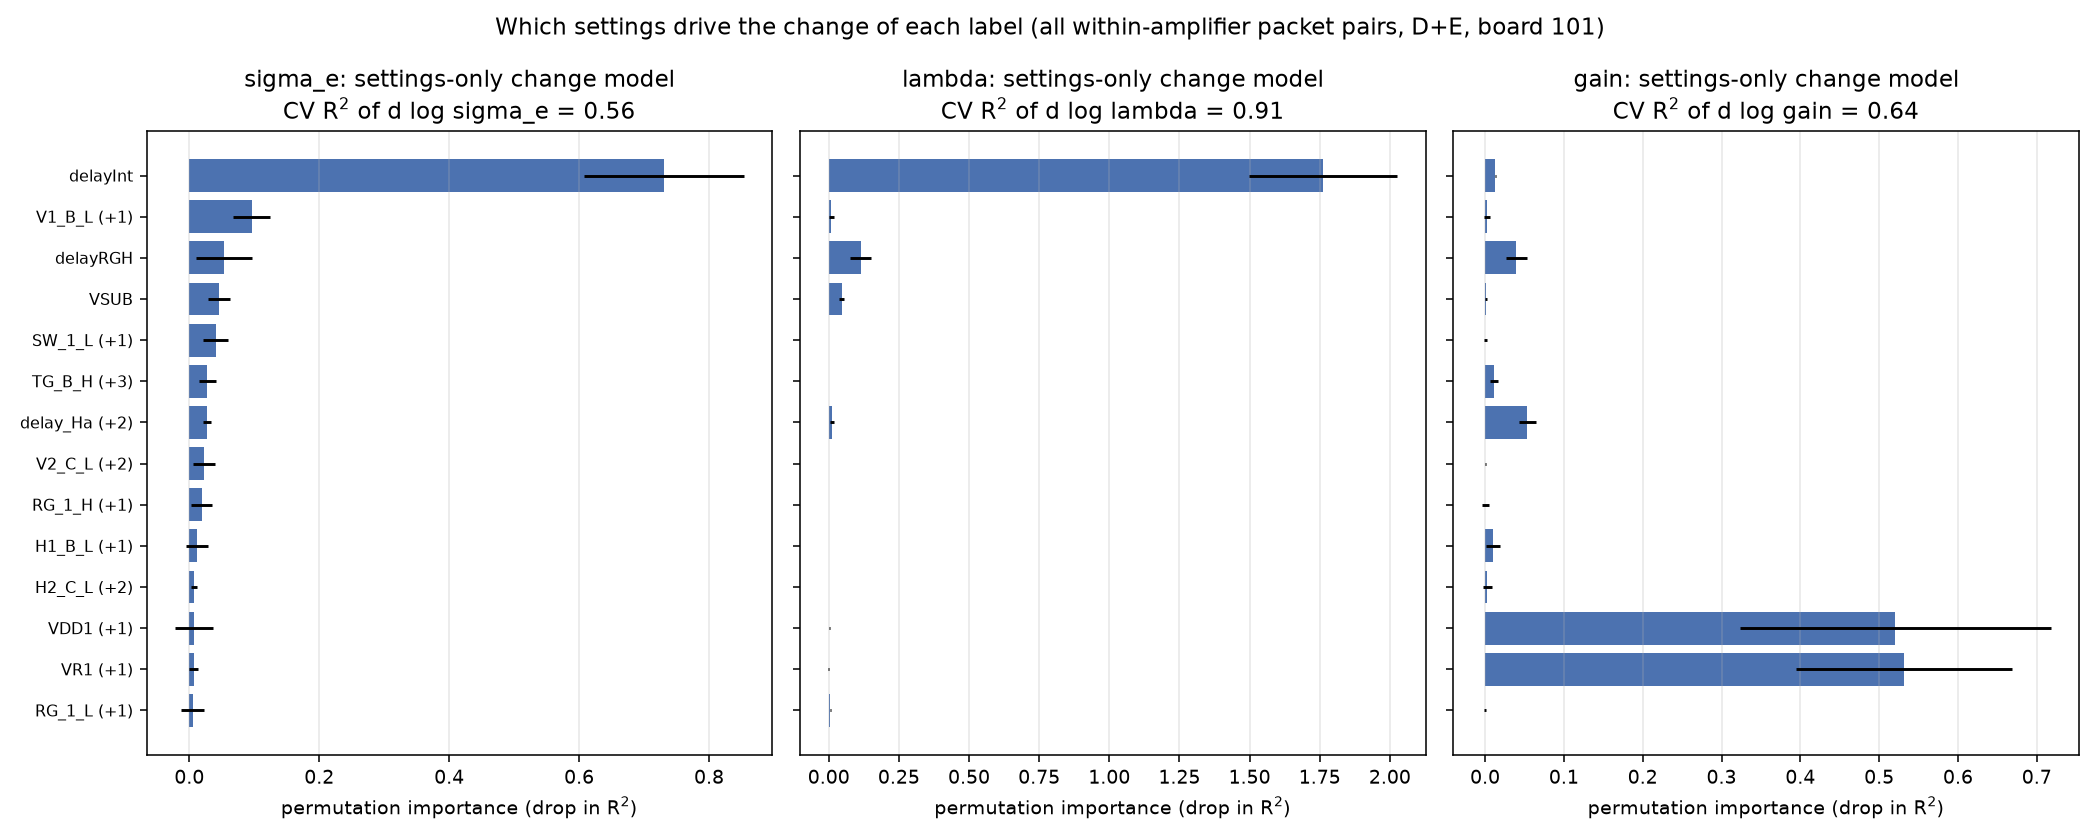
\includegraphics[width=\textwidth]{figures/knob_importance.png}
\caption{Which settings drive the change of each label (v2, all within-amplifier packet pairs): permutation importance of
a settings-only change model. $\lambda$: \texttt{delayInt}; gain: VR, VDD; $\sigma_e$: \texttt{delayInt}, then several voltages.}
\label{fig:importance}
\end{figure}

\begin{figure}[ht]\centering
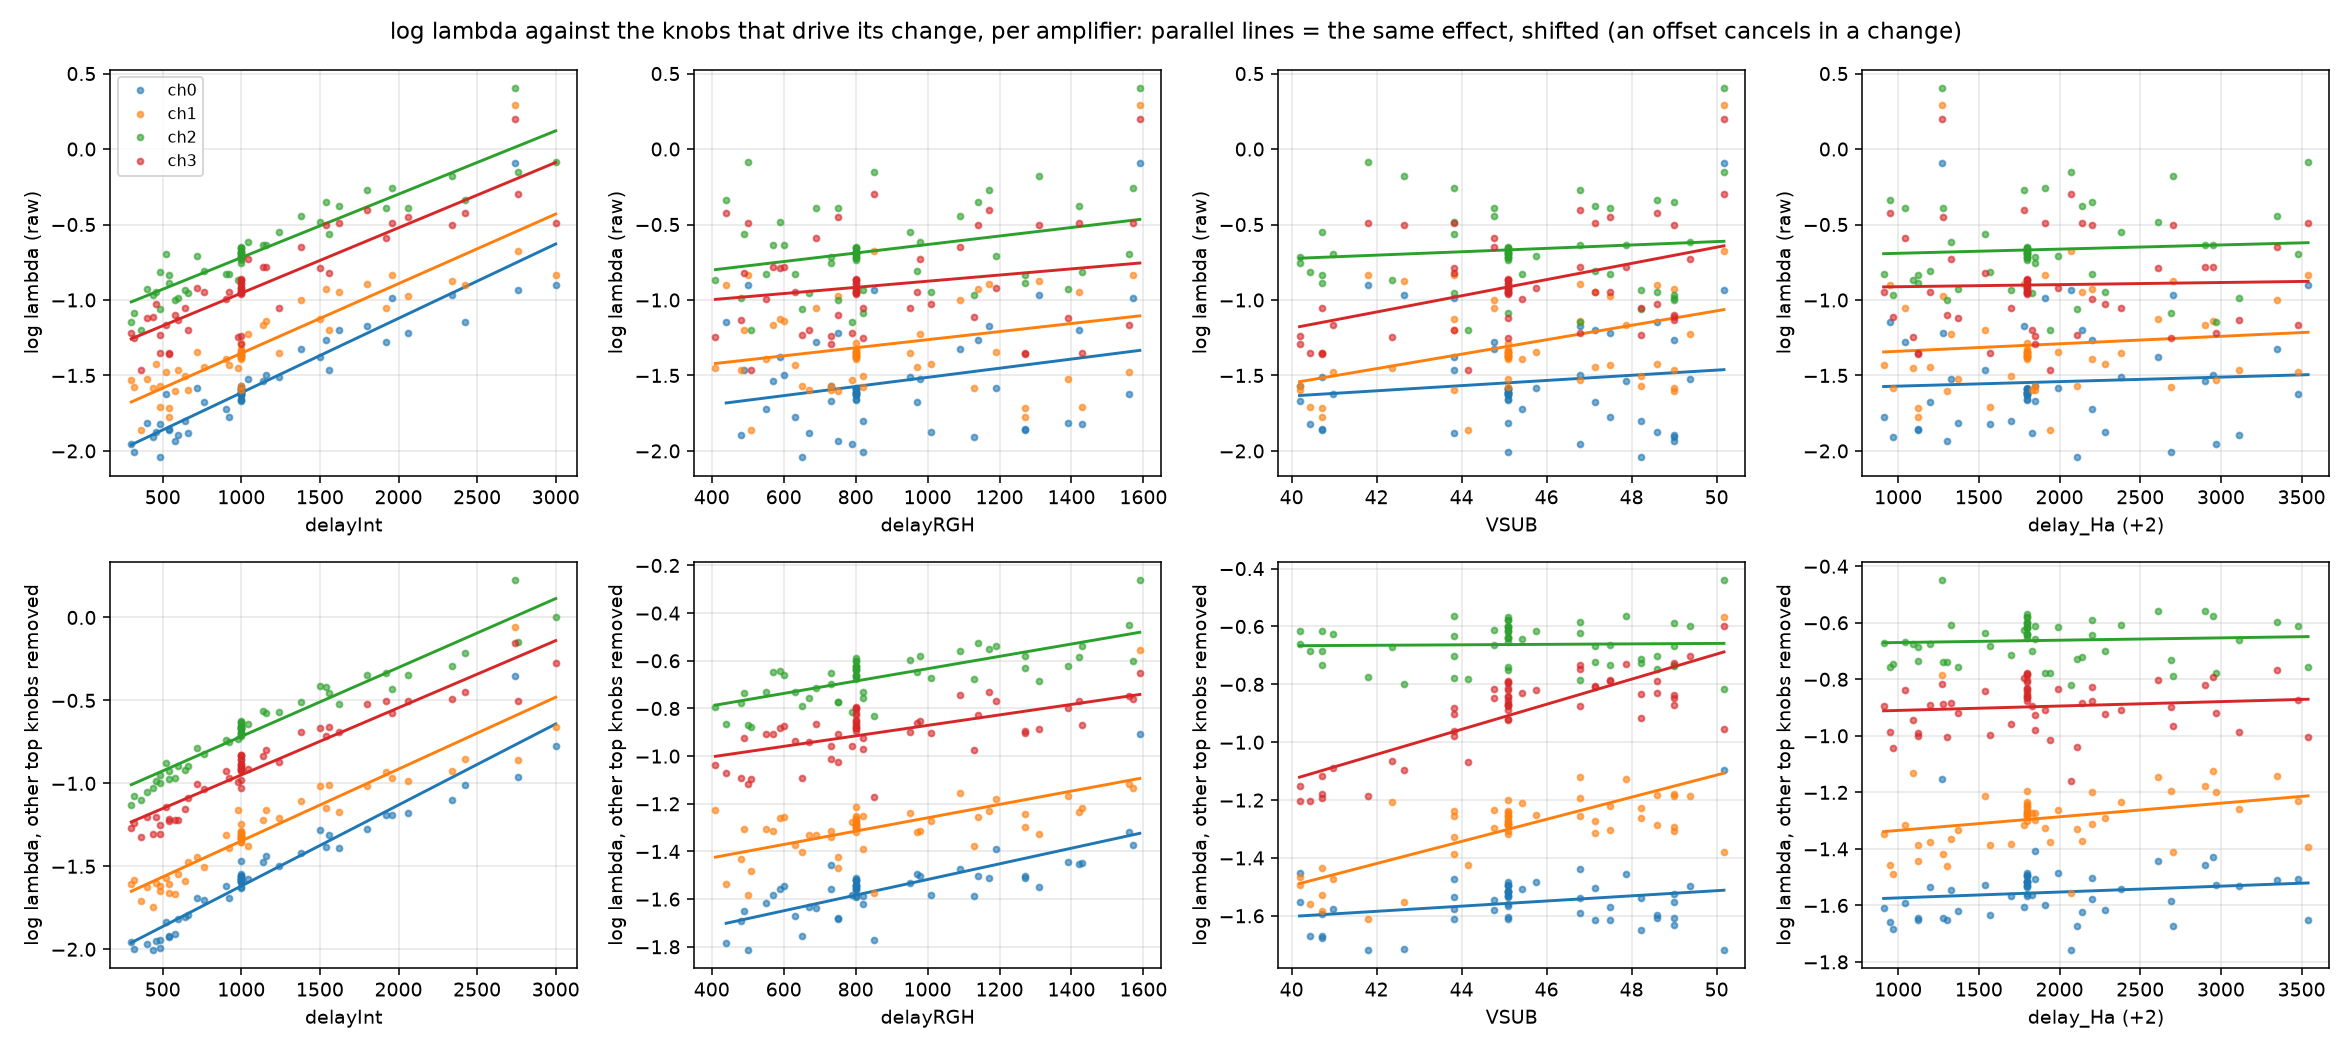
\includegraphics[width=\textwidth]{figures/lambda_vs_knobs.png}
\caption{$\log\lambda$ against the top knobs, per amplifier (bottom: the other top knobs removed). Parallel lines: the same
effect, a different offset per amplifier. VSUB: steep on ch1 and ch3, flat on ch0 and ch2.}
\label{fig:lambdaknobs}
\end{figure}

\begin{figure}[ht]\centering
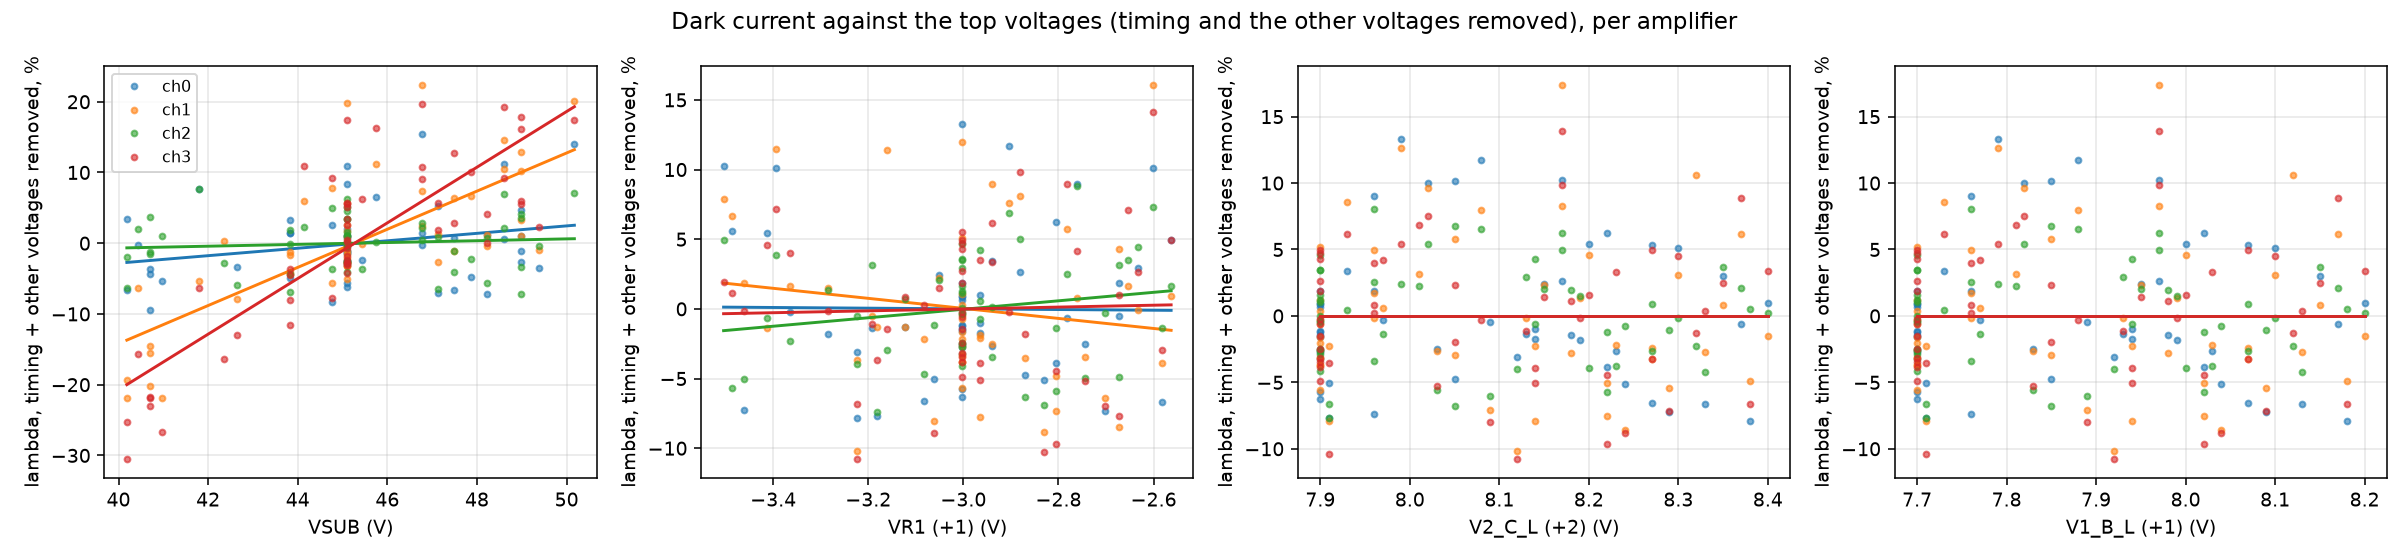
\includegraphics[width=\textwidth]{figures/voltage_partial.png}
\caption{Dark current against the top voltages with the timing and the other voltages removed (v2, L2\_72 left out).
Only VSUB shows an effect clearly above the scatter; V1 and V2 lows moved in lockstep and cannot be separated.}
\label{fig:volts}
\end{figure}

\begin{figure}[ht]\centering
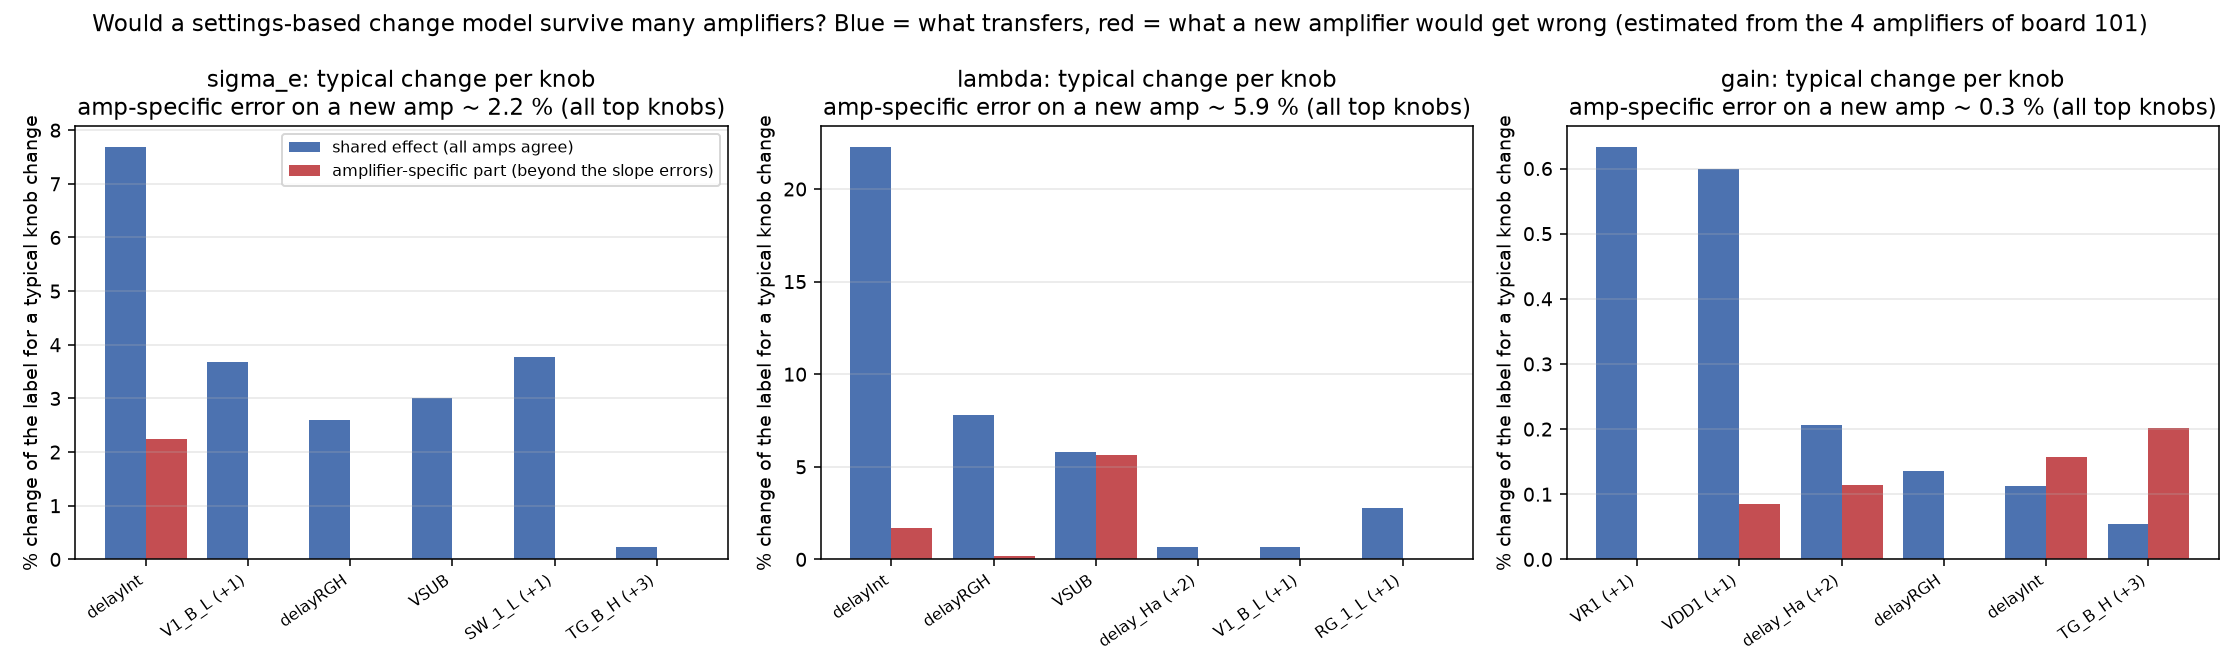
\includegraphics[width=\textwidth]{figures/amp_transfer.png}
\caption{Per knob, the change all amplifiers share (blue) against the amplifier-specific part (red): what a change model
gets wrong on an amplifier it has not seen. VSUB is the risk for $\lambda$.}
\label{fig:transfer}
\end{figure}

\section{The goals of v3}

\subsection{The voltages and the dark current (the user's goal, 2026-11-10)}
In the user's words: in the next training data a large subset should be focused on \emph{voltage-only} changes, to train
more on how the dark current changes with the voltage settings. If the timing is increased or decreased, the dark current
goes up and down with the readout time; the more subtle and more interesting question is how a change of the
\emph{voltages} affects the dark current. v3 therefore keeps the timing at nominal for most packets and varies the
voltages as widely as the windows and the rules allow.

\subsection{Quantify the influence of every parameter (new project goal)}
Next to training the models, a goal of the project is now to quantify \emph{how much each parameter influences the noise
and the dark current}: for every knob, its effect per volt (or per doubling of a time), with an uncertainty; its share of
the variance over the operating range; its interactions with the other knobs; how much it differs between amplifiers;
and for $\lambda$, whether it acts on the dark-current rate or on the clock-induced charge. The analysis is
\texttt{lvl1/parameter\_influence.py} (Section~\ref{sec:analysis}); it runs on v2 today and on v3 when it is taken.

\subsection{The models}
Train and test the level-1 models (absolute and change, traces, strips, settings, hybrids) on v3 as on v2, with the
emphasis on changes at fixed timing; measure how the v2-trained models extrapolate to v3's wider voltages.

\section{The v3 data set}

\subsection{Sessions and blocks}
\begin{center}
\begin{tabular}{llrrl}
\toprule
session & block & packets & time & what it is for\\
\midrule
G & voltage Sobol & 38 & 10.0\,h & all 15 voltage groups jointly, nominal timing\\
G & one at a time & 33 & 8.7\,h & each group to its lowest and highest allowed value; midpoints for V1\_L, H1\_L,\\
  & & & & the two swings and TG; VSUB at 35, 40, 50, 57.5, 70\,V\\
G & voltage $\times$ timing & 25 & 8.0\,h & voltage Sobol points at \texttt{delayInt} 500 and 2500 (12 each)\\
G & corner & 9 & 3.0\,h & factorial: \texttt{delayRGH} 1500 alone, VSUB 65\,V alone, both; at \texttt{delayInt} 500, 1000, 2500\\
G & nominal & 18 & 4.7\,h & drift and label noise (4 earlier points are also repeated)\\
H & voltage Sobol + voltage $\times$ timing & 24 & 6.6\,h & prospective test, scored once after the freeze\\
H & nominal & 5 & 1.3\,h & drift\\
\midrule
all & & 152 & 42.3\,h & \\
\bottomrule
\end{tabular}
\end{center}
Every second session-G packet that follows a non-nominal one takes its reference at the previous packet's settings
(43 packets), so many within-packet changes are voltage $\to$ voltage at fixed timing and go both ways. A nominal packet
every 7 packets tracks the drift; four earlier design points are repeated later (label noise away from nominal). The
order is shuffled. Every \texttt{delayInt} is a multiple of 20 cycles (whole ADC samples: no fractional-window labels).

\subsection{The voltage box}
Each group is sampled over its window of \texttt{configs/limits.toml}, cut by the relationship rules with a 0.5\,V
margin and by a minimum clock swing of 1.5\,V (the range below is that of the group alone, all else nominal; joint points
must also pass and are redrawn otherwise). The clock \emph{highs} are sampled as a swing: each high follows its own low,
plus the swing change, so the low level and the swing (high $-$ low) are separate knobs.
\begin{center}
\begin{tabular}{lllll}
\toprule
group & pins & nominal & v3 range & v2\\
\midrule
VSUB & VSUB & 45 & $-10$ to $+25$\,V (35--70\,V) & $\pm 5$\\
VDD & VDD1, VDD2 & $-19$ & $\pm 2$\,V & $\pm 1$\\
VR & VR1, VR2 & $-3$ & $\pm 1$\,V & $\pm 0.5$\\
RG\_H, RG\_L & RG\_1/2\_H, \_L & 9, 3 & $-2$ to $+1$, $\pm 2$\,V & $\pm 0.5$\\
SW\_L & SW\_1/2\_L & $-6$ & $-2$ to $-0.5$\,V (or nominal) & $-0.5$ to 0\\
V1, V2, V3 lows (each) & V*\_L & 7.7--7.9 & 0 to $+0.5$\,V & 0 to $+0.5$, locked\\
V swing & V*\_H & 9.9 (swing 2.0--2.2) & $-0.5$ to $+0.1$\,V & never varied\\
H1, H2, H3 lows (each) & H*\_L & 6.5--6.7 & $-1.3$ ($-1.5$) to $+0.2$\,V & $\pm 0.5$, locked\\
H swing & H*\_H & 9.0--9.5 & $-0.8$ to $+0.5$\,V & never varied\\
TG & TG\_A/B\_H/L & 7.4 & $-0.2$ to 0\,V & $\pm 0.25$\\
\bottomrule
\end{tabular}
\end{center}
The A and B halves of the CCD and both readout stages move together (both sides keep their nominal offsets).
\textbf{The 0.5\,V margin narrows the vertical clocks and TG:} at nominal, V1\_B\_L and V3\_B\_L (7.7\,V) are only 0.3\,V
above TG (7.4\,V), so the V lows can only go up and TG only down a little; the V-low effects are measured on the upper
side only. The H lows, the swings, VSUB and the readout-stage rails keep wide ranges.

\subsection{Safety: the windows and the relationship rules}
The rules that must hold are the voltage windows of \texttt{configs/limits.toml} and the group's relationship rules
(\texttt{docs/voltage\_rules.txt}, enforced in \texttt{src/ccd\_limits.py}): every clock high at or above its low;
VDD $>$ VDRAIN; SW\_H $>$ OG\_H; DG\_H $>$ VR; DG\_L $<$ VR; OG\_L $<$ VR; OG\_L $\geq$ SW\_L; V clock lows above every TG
level; H clock lows below every TG level; H3 lows above SW\_H; VDRAIN $<$ DG\_L; VDD below VR. On top of the rules
(2026-11-10, the user and the review):
\begin{itemize}
\item \textbf{0.5\,V margin} on every relationship a packet changes (a relation left exactly as at nominal is allowed);
\item \textbf{clock swing $\geq$ 1.5\,V} on every V and H clock (sampled independently, the V swing fell below 1\,V in
  most packets of the first draft, which would break the parallel transfer);
\item \textbf{ramps:} \texttt{manual\_packet.sh} applies a changes file one line at a time; large changes are written as
  ramps (VSUB in steps of at most 5\,V, every other voltage in steps of its \texttt{max\_step}: 0.5\,V for the clocks,
  1\,V for VDD), all pins moving together, and within a step the pins are sent in an order that keeps every intermediate
  configuration inside the windows and the rules;
\item \textbf{the way back:} every changes file has an \texttt{\_undo.txt} file, the ramped, rule-safe way back to
  nominal. The reset at the end of a packet reloads the module's \texttt{.bcf}, which restores the pins in an order we do
  not control (after a TG change it can put a TG high briefly below its TG low); sending the undo file just before the
  reset makes the reset a no-op. \textbf{\texttt{manual\_packet.sh} does not do this yet.}
\end{itemize}
The v1/v2 restriction ``every voltage within one \texttt{max\_step} of nominal'' was dropped (2026-11-10, the user):
\texttt{max\_step} in \texttt{limits.toml} is the step of a ramp, not a limit on the range. All 367 files (152 packets,
43 reference files and their undo files) were replayed line by line: no intermediate state breaks a rule; the smallest
clock swing is 1.50\,V; the largest single step is 1.0\,V (5\,V for VSUB). VSUB 35--70\,V is confirmed by the user.

\subsection{What changes from v2, and why}
\begin{itemize}
\item \textbf{Voltage-only packets} (72 of 123 against 13 of 52 at nominal timing): the timing hides the voltages.
\item \textbf{Independent clock phases} (V1, V2, V3 lows apart; H1, H2, H3 lows apart): v2's locked groups cannot be
  separated.
\item \textbf{Clock swings varied} (the highs follow their lows, plus a swing change, swing $\geq$ 1.5\,V): the effect of
  a clock's \emph{level} can be told from that of its \emph{swing} (surface dark current against clock-induced charge).
\item \textbf{Whole windows instead of one max\_step}: effects of a few \% per volt only rise above the 2.5\,\% label
  noise of $\lambda$ over ranges of 1--2\,V.
\item \textbf{One-at-a-time sweeps}: model-free single effects to check the joint fits against.
\item \textbf{Voltage $\times$ timing} (12 points each at \texttt{delayInt} 500 and 2500, against the nominal-timing
  block): a voltage effect that scales with the readout time is a dark-current rate effect, one that does not is
  clock-induced charge.
\item \textbf{The corner as a factorial} (\texttt{delayRGH} high alone, VSUB high alone, both, at three
  \texttt{delayInt}): the interaction that broke the $\lambda$ prediction on E, separated from the main effects.
\end{itemize}

\section{Quantifying the influence of each parameter}\label{sec:analysis}
\texttt{lvl1/parameter\_influence.py} (any processed data set; every number with an uncertainty; log units, so every
effect is a \% change):
\begin{enumerate}
\item[A] \textbf{Effects:} a linear model per amplifier and pooled (one offset per amplifier, shared slopes), \% per volt
  (per doubling for a time) and per standard deviation, 68\,\% bootstrap intervals over packets.
\item[B] \textbf{Importance:} boosted trees on the knobs and the amplifier; cross-validated $R^2$ (grouped by packet),
  permutation importance, partial dependence of the top knobs per amplifier (non-linear shapes).
\item[C] \textbf{Variance shares (Sobol indices)} over the operating box from the tree surrogate: each knob's share alone
  (first order) and with its interactions (total order).
\item[D] \textbf{One at a time:} packets one knob away from nominal against the nominal packets interpolated in time on the
  same amplifier: a model-free effect with the nominal scatter as its error.
\item[E] \textbf{Amplifiers:} the effect all amplifiers share against the amplifier-specific part (what transfers).
\item[F] \textbf{Dark-current rate against clock-induced charge} ($\lambda$): $\lambda = t^{\alpha}\exp(r_a + \sum_k r_k z_k)
  + \exp(c_a + \sum_k c_k z_k)$ over the voltages $z_k$, $t$ the skip-cycle time.
\item[G] \textbf{Level against swing} for clocks whose high and low were both varied.
\end{enumerate}
Companion figures: \texttt{lvl1/lambda\_settings\_figures.py} (importance, per-amplifier lines, transfer, residuals) and
\texttt{lvl1/voltage\_dark\_current.py} (the voltages with the timing removed). First results on v2 are in Section 1.2 and
Figs.~\ref{fig:influence}--\ref{fig:influencesig}.

\begin{figure}[ht]\centering
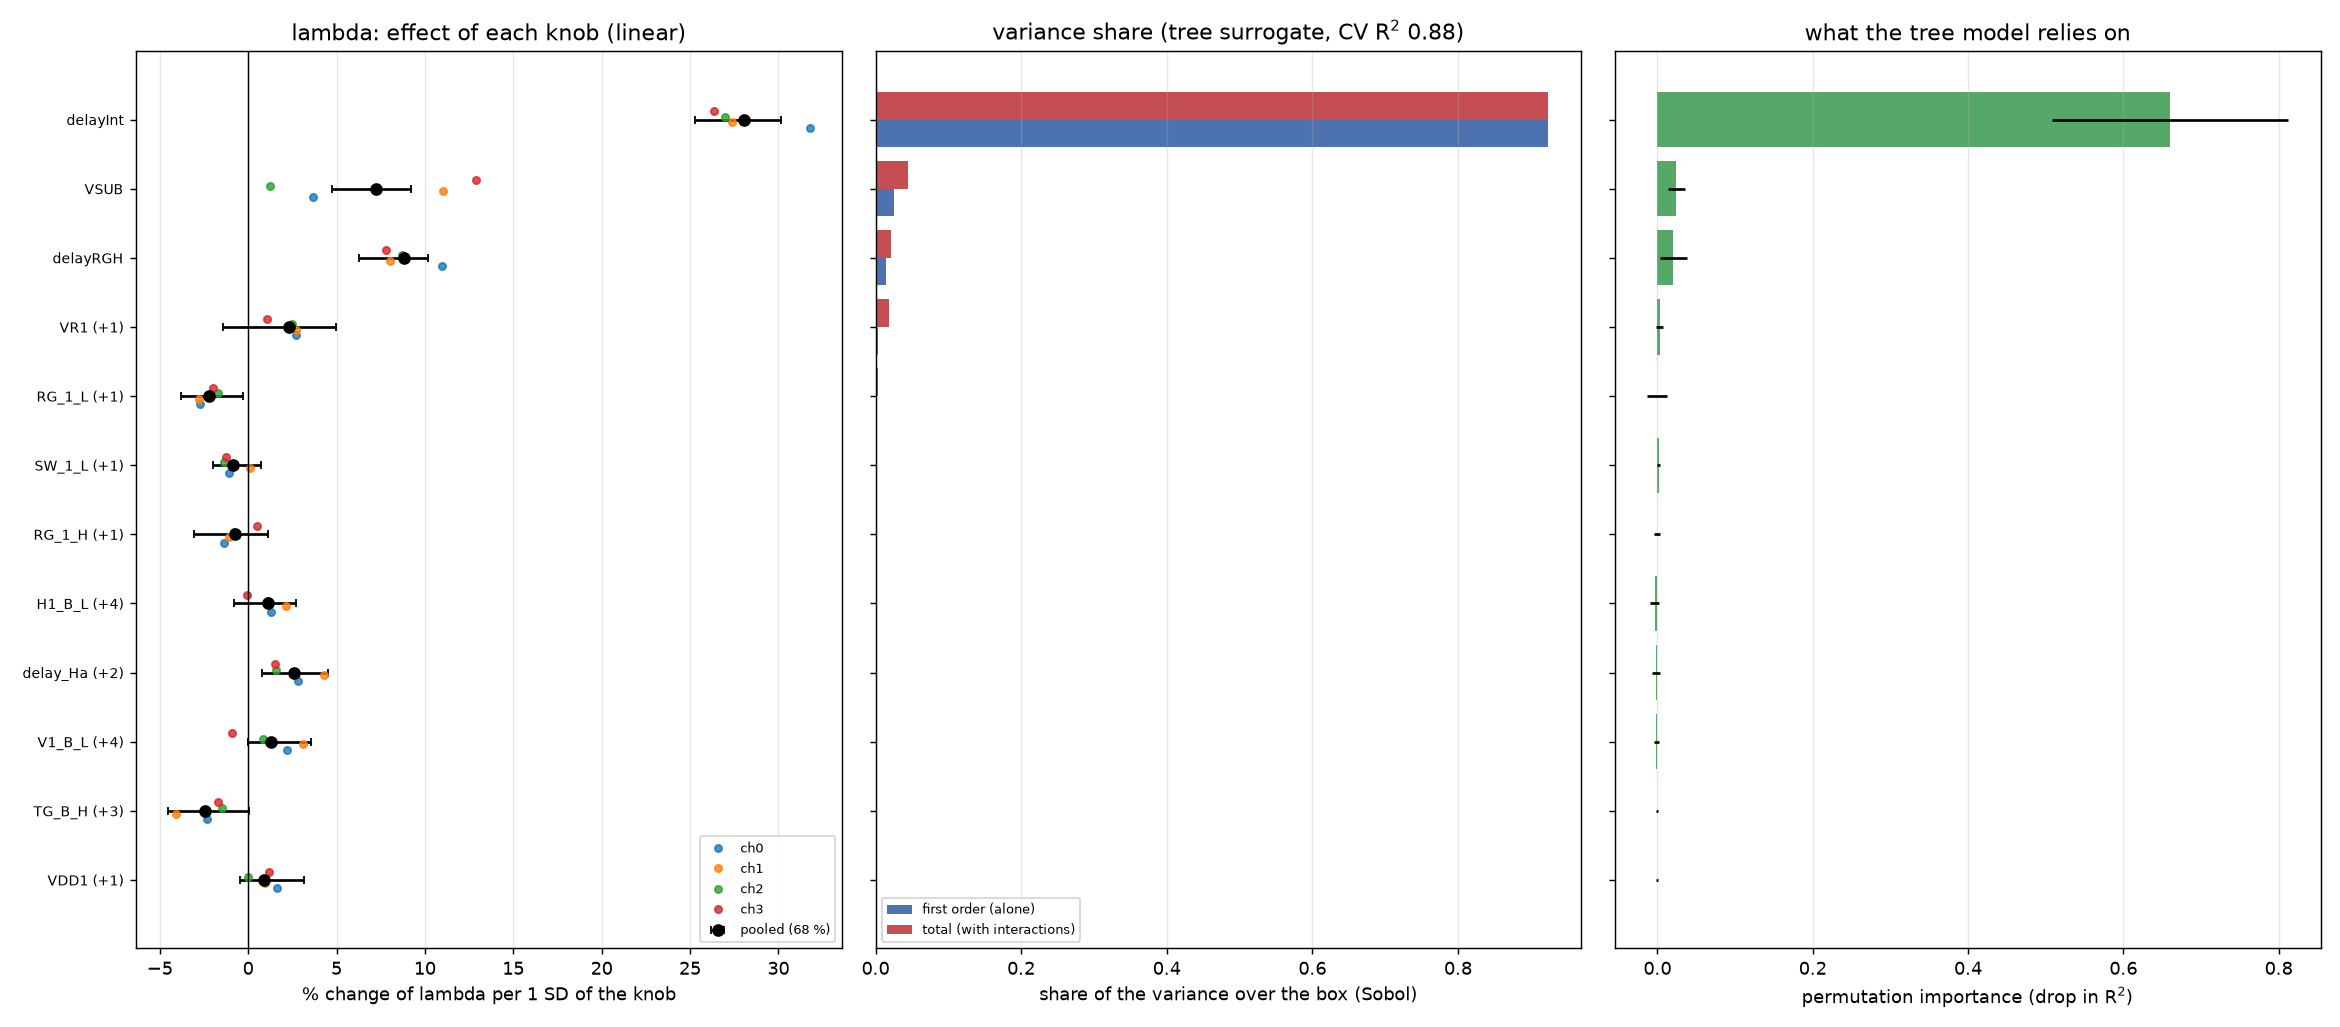
\includegraphics[width=\textwidth]{figures/influence_lambda.png}
\caption{$\lambda$ on v2: effect per knob (pooled and per amplifier), variance shares (Sobol), permutation importance.}
\label{fig:influence}
\end{figure}
\begin{figure}[ht]\centering
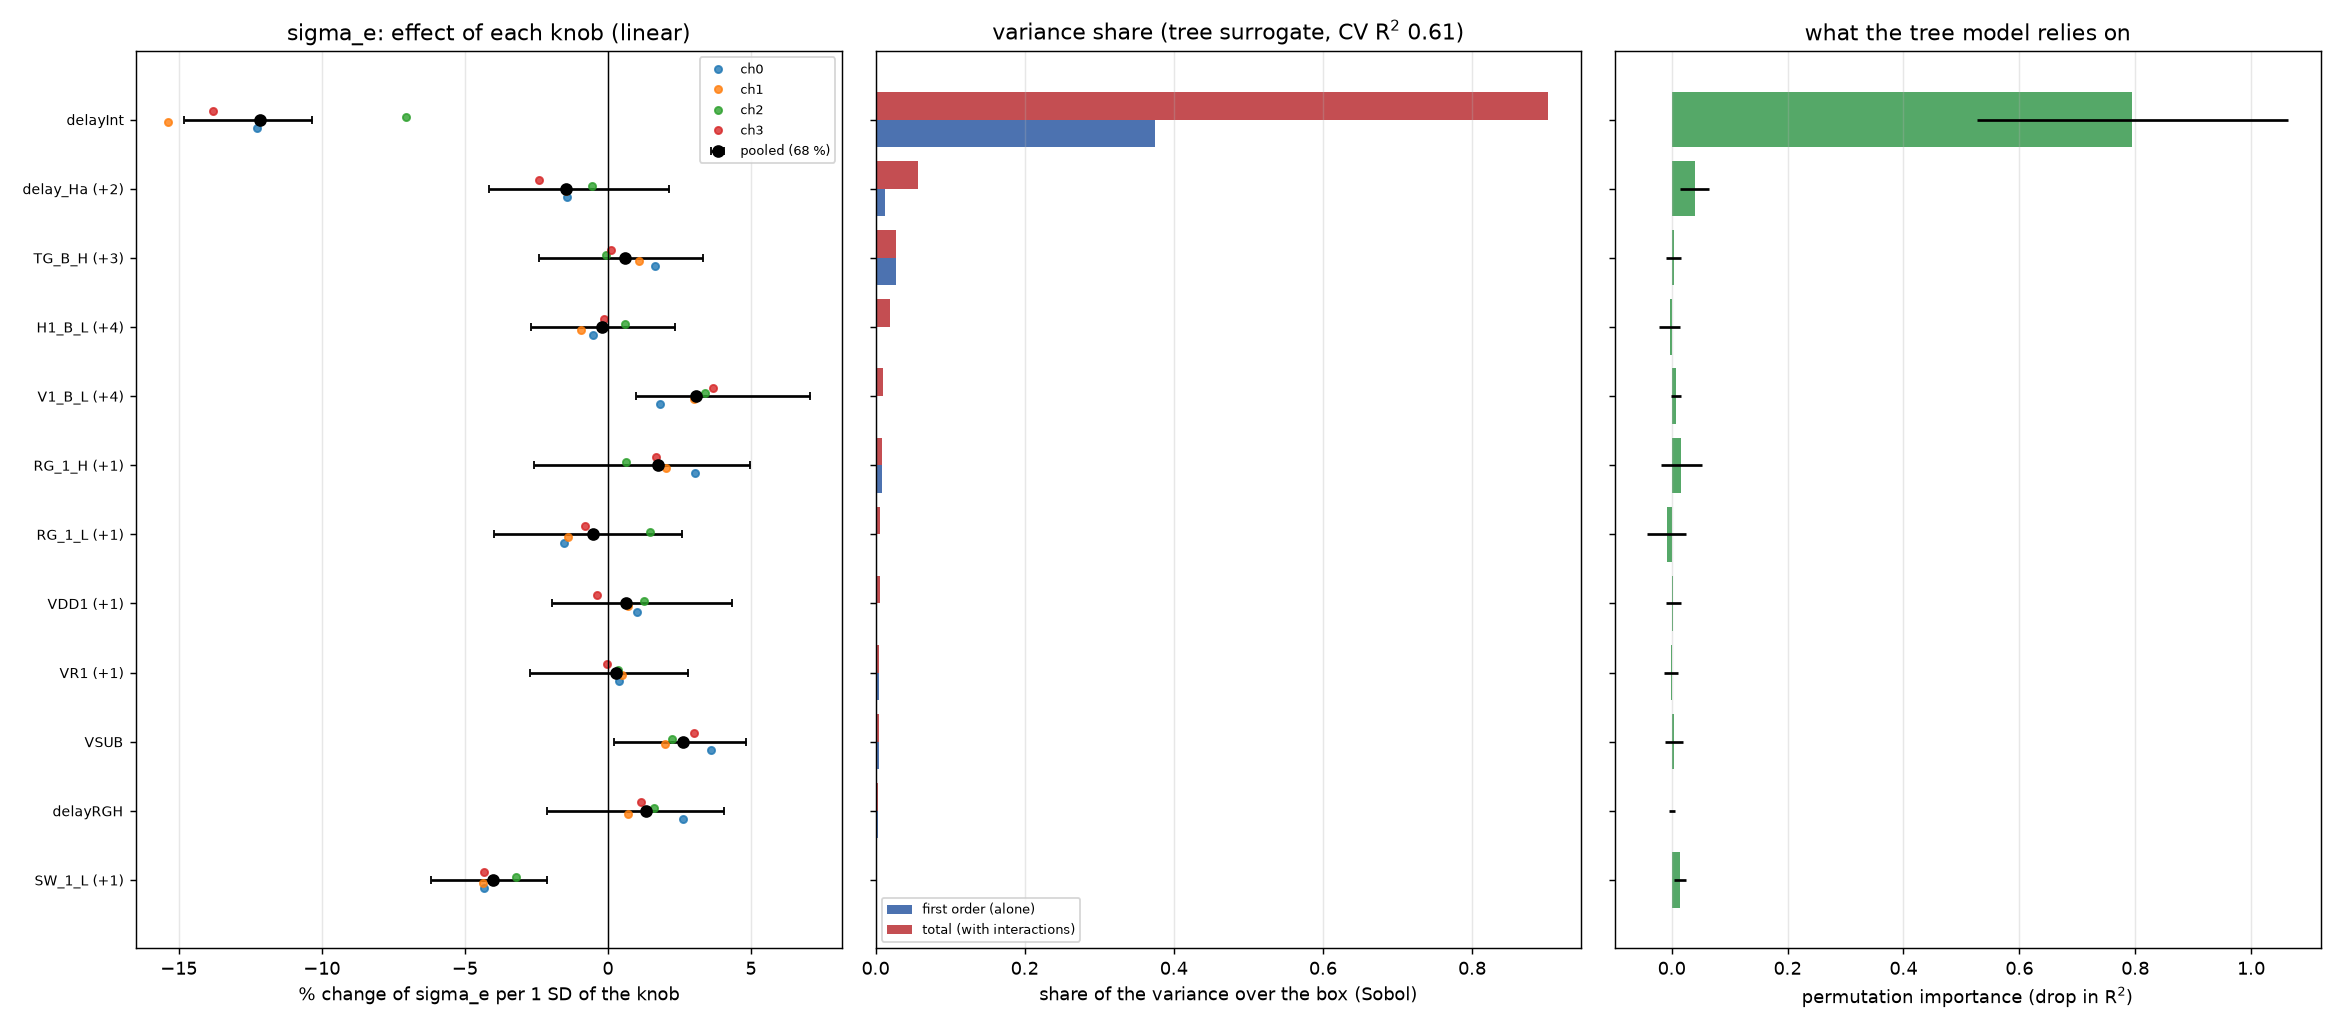
\includegraphics[width=\textwidth]{figures/influence_sigma_e.png}
\caption{$\sigma_e$ on v2. \texttt{delayInt}'s total share (0.90) is far above its first-order share (0.38): its effect is
strongly non-linear and depends on the other knobs.}
\label{fig:influencesig}
\end{figure}

\section{The models on v3}
\begin{itemize}
\item \textbf{Protocol as v2:} setting-grouped cross-validation on G for every model and source; freeze the choice
  (written to git) before H is scored; H scored once, with paired bootstraps against the settings-only references.
  Pass mark: direction of clear changes $\geq 90$\,\% on amplifiers not in training.
\item \textbf{Change models} train on within-packet (image), strip, $n \to n{+}1$, $n \to n{+}2$ and random pairs within
  one amplifier (never across amplifiers or sessions); scored separately on pairs \emph{at fixed timing} (the new
  emphasis) and pairs with a timing change.
\item \textbf{Hybrids:} the settings change corrected by the traces (combined trees, residual trees, direction
  classifier) and averages of the trace models; the trace change GP is dropped (it collapsed and took 40--90\,min).
\item \textbf{Extrapolation:} the v2-trained models scored on v3 before retraining (how they fail outside their range).
\item \textbf{$\lambda$:} train change models on the timing-corrected $\lambda$ as well, with an amplifier-specific VSUB term.
\end{itemize}

\section{What v3 should answer}
\begin{enumerate}
\item Which voltages move the dark current, by how much per volt, and whether linearly or past a threshold.
\item Whether each acts on the dark-current rate or on the clock-induced charge, and through the clock level or the swing.
\item Which effects are the same on every amplifier and which are amplifier-specific (VSUB in v2).
\item The same for the noise: which voltages move $\sigma_e$ at fixed timing.
\item Whether a settings model predicts voltage-driven $\lambda$ changes as well as timing-driven ones (expected: worse),
  and whether the traces or the hybrids add information there.
\item Whether training on fixed-timing changes lifts the $\sigma_e$ direction above 74\,\% (pass mark 90\,\%).
\end{enumerate}
If almost no voltage besides VSUB moves $\lambda$ even over the wider windows, that too is an answer: the operating-point
search for the dark current is then essentially timing + VSUB, and the traces matter mainly for the noise.

\section{Review and before taking it}
An independent review of the first draft (2026-11-10) found the line-by-line rule checks clean but asked for changes; all
are in the plan above: the vertical swing (it collapsed below 1\,V in most packets when the highs were sampled
independently: now a swing knob with a 1.5\,V minimum), the margins (now 0.5\,V), ramps for large jumps, the way back to
nominal (undo files), a larger voltage $\times$ timing block (the rate/CIC split was under-determined with 15 packets),
the corner as a factorial, midpoints in the one-at-a-time sweeps, a larger test session, and no two nominal packets in a
row. Still open:
\begin{itemize}
\item \textbf{\texttt{manual\_packet.sh}} should send \texttt{<id>\_undo.txt} (and \texttt{<id>\_ref\_undo.txt}) before
  its reset to nominal, so the \texttt{.bcf} reload starts from nominal and cannot cross a rule;
\item \texttt{configs/limits.toml} still says \texttt{reviewed = false}: the user has confirmed VSUB 35--70\,V and the
  other windows;
\item the one-at-a-time ends are single packets (one shot carries about 3.5\,\% noise on $\lambda$: effects below about
  7\,\% need the joint fits);
\item record the CCD temperature per packet if a readout exists ($\lambda$ drifts);
\item the image TOML (\texttt{image\_params/tc1/img32.toml}) on the DAQ machine, as for v2.
\end{itemize}

\section{Commands}
\begin{Verbatim}
python lvl1/make_packet_plan_v3.py                     # the plan: lvl1/packet_plan_v3/ (PLAN.md, plan.json, L3_NNN.txt)
DRY_RUN=1 PLAN_DIR=lvl1/packet_plan_v3 bash daq_scripts/run_plan.sh
PLAN_DIR=lvl1/packet_plan_v3 bash daq_scripts/run_plan.sh
# after processing (processed_v3):
.venv/bin/python lvl1/parameter_influence.py --data processed_v3 --plan lvl1/packet_plan_v3/plan.json \
    --sessions G --out processed_v3/lvl1_results/parameter_influence
.venv/bin/python lvl1/scorecard_v2.py --data processed_v3 --plan lvl1/packet_plan_v3/plan.json --train-session G \
    --out processed_v3/lvl1_results/scorecard_G          # after the freeze: --holdout-session H
.venv/bin/python lvl1/voltage_dark_current.py --data processed_v3 --plan lvl1/packet_plan_v3/plan.json --sessions G \
    --out processed_v3/lvl1_results/voltages
\end{Verbatim}

\end{document}
